\documentclass[a4paper,11pt]{exam}
\printanswers % pour imprimer les réponses (corrigé)
%\noprintanswers % Pour ne pas imprimer les réponses (énoncé)
\addpoints % Pour compter les points
% \noaddpoints % pour ne pas compter les points
%\qformat{\textbf{\thequestion ) } }
%\qformat{\textbf{\thequestion )}} % Pour définir le style des questions (facultatif)
\usepackage{color} % définit une nouvelle couleur
\shadedsolutions % définit le style des réponses
% \framedsolutions % définit le style des réponses
\definecolor{SolutionColor}{rgb}{0.8,0.9,1} % bleu ciel
\renewcommand{\solutiontitle}{\noindent\textbf{Solution:}\par\noindent} % Définit le titre des solutions




\makeatletter

\def\maketitle{{\centering%
	\par{\huge\textbf{\@title}}%
	\par{\@date}%
	\par}}


\renewcommand{\thesubsection}{\Alph{subsection}.}   

\makeatother

\lhead{NOM Pr\'enom :}
\rhead{\textbf{Les r\'eponses doivent \^etre justifi\'ees et r\'edig\'ees}}
\cfoot{\thepage / \pageref{LastPage}}


%\usepackage{../../pas-math}
%\usepackage{../../moncours}


%\usepackage{pas-cours}
%-------------------------------------------------------------------------------
%          -Packages nécessaires pour écrire en Français et en UTF8-
%-------------------------------------------------------------------------------
\usepackage[utf8]{inputenc}
\usepackage[frenchb]{babel}
%\usepackage{numprint}
\usepackage[T1]{fontenc}
%\usepackage{lmodern}
\usepackage{textcomp}
\usepackage[french, boxed]{algorithm2e}
\usepackage{hyperref}


%-------------------------------------------------------------------------------

%-------------------------------------------------------------------------------
%                          -Outils de mise en forme-
%-------------------------------------------------------------------------------
\usepackage{hyperref}
\hypersetup{pdfstartview=XYZ}
%\usepackage{enumerate}
\usepackage{graphicx}
\usepackage{multicol}
\usepackage{tabularx}
\usepackage{multirow}
\usepackage{color}
\usepackage{eurosym}


\usepackage{anysize} %%pour pouvoir mettre les marges qu'on veut
%\marginsize{2.5cm}{2.5cm}{2.5cm}{2.5cm}

\usepackage{indentfirst} %%pour que les premier paragraphes soient aussi indentés
\usepackage{verbatim}
\usepackage{enumitem}
\usepackage{booktabs}
\usepackage[usenames,dvipsnames,svgnames,table]{xcolor}

\usepackage{variations}

%-------------------------------------------------------------------------------


%-------------------------------------------------------------------------------
%                  -Nécessaires pour écrire des mathématiques-
%-------------------------------------------------------------------------------
\usepackage{amsfonts}
\usepackage{amssymb}
\usepackage{amsmath}
\usepackage{amsthm}
\usepackage{tikz}
\usepackage{xlop}
\usepackage[output-decimal-marker={,}]{siunitx}
%-------------------------------------------------------------------------------

%-------------------------------------------------------------------------------
%                  -Nécessaires pour écrire des formules chimiquess-
%-------------------------------------------------------------------------------

\usepackage[version=4]{mhchem}

%-------------------------------------------------------------------------------
% Pour pouvoir exploiter les fichiers directement dans beamer
\newcommand{\pause}{\ }
%-------------------------------------------------------------------------------
%                    - Mise en forme avancée
%-------------------------------------------------------------------------------

\usepackage{ifthen}
\usepackage{ifmtarg}


\newcommand{\ifTrue}[2]{\ifthenelse{\equal{#1}{true}}{#2}{$\qquad \qquad$}}

%\newcommand{\kword}[1]{\textcolor{red}{\underline{#1}}}
%-------------------------------------------------------------------------------

%-------------------------------------------------------------------------------
%                     -Mise en forme d'exercices-
%-------------------------------------------------------------------------------
%\newtheoremstyle{exostyle}
%{\topsep}% espace avant
%{\topsep}% espace apres
%{}% Police utilisee par le style de thm
%{}% Indentation (vide = aucune, \parindent = indentation paragraphe)
%{\bfseries}% Police du titre de thm
%{.}% Signe de ponctuation apres le titre du thm
%{ }% Espace apres le titre du thm (\newline = linebreak)
%{\thmname{#1}\thmnumber{ #2}\thmnote{. \normalfont{\textit{#3}}}}% composants du titre du thm : \thmname = nom du thm, \thmnumber = numéro du thm, \thmnote = sous-titre du thm

%\theoremstyle{exostyle}
%\newtheorem{exercice}{Exercice}
%
%\newenvironment{questions}{
%\begin{enumerate}[\hspace{12pt}\bfseries\itshape a.]}{\end{enumerate}
%} %mettre un 1 à la place du a si on veut des numéros au lieu de lettres pour les questions 
%-------------------------------------------------------------------------------

%-------------------------------------------------------------------------------
%                    - Mise en forme de tableaux -
%-------------------------------------------------------------------------------

\renewcommand{\arraystretch}{1.7}

\setlength{\tabcolsep}{1.2cm}

%-------------------------------------------------------------------------------



%-------------------------------------------------------------------------------
%                    - Racourcis d'écriture -
%-------------------------------------------------------------------------------
%Droites
\newcommand{\dte}[1]{$(#1)$}
\newcommand{\fig}[1]{figure $#1$}
\newcommand{\sym}{symétrique}
\newcommand{\syms}{symétriques}
\newcommand{\asym}{axe de symétrie}
\newcommand{\asyms}{axes de symétrie}
\newcommand{\seg}[1]{$[#1]$}
\newcommand{\monAngle}[1]{$\widehat{#1}$}
\newcommand{\bissec}{bissectrice}
\newcommand{\mediat}{médiatrice}
\newcommand{\ddte}[1]{$[#1)$}


% Angles orientés (couples de vecteurs)
\newcommand{\aopp}[2]{(\vec{#1}, \vec{#2})} %Les deuc vecteurs sont positifs
\newcommand{\aopn}[2]{(\vec{#1}, -\vec{#2})} %Le second vecteur est négatif
\newcommand{\aonp}[2]{(-\vec{#1}, \vec{#2})} %Le premier vecteur est négatif
\newcommand{\aonn}[2]{(-\vec{#1}, -\vec{#2})} %Les deux vecteurs sont négatifs

%Ensembles mathématiques
\newcommand{\naturels}{\mathbb{N}} %Nombres naturels
\newcommand{\relatifs}{\mathbb{Z}} %Nombres relatifs
\newcommand{\rationnels}{\mathbb{Q}} %Nombres rationnels
\newcommand{\reels}{\mathbb{R}} %Nombres réels
\newcommand{\complexes}{\mathbb{C}} %Nombres complexes


%Intégration des parenthèses aux cosinus
\newcommand{\cosP}[1]{\cos\left(#1\right)}
\newcommand{\sinP}[1]{\sin\left(#1\right)}


%Probas stats
\newcommand{\stat}{statistique}
\newcommand{\stats}{statistiques}


\newcommand{\homo}{homothétie}
\newcommand{\homos}{homothéties}


\newcommand{\mycoord}[3]{(\textcolor{red}{\num{#1}} ; \textcolor{Green}{\num{#2}} ; \textcolor{blue}{\num{#3}})}
%-------------------------------------------------------------------------------

%-------------------------------------------------------------------------------
%                    - Mise en page -
%-------------------------------------------------------------------------------

\newcommand{\twoCol}[1]{\begin{multicols}{2}#1\end{multicols}}


\setenumerate[1]{font=\bfseries,label=\textit{\alph*})}
\setenumerate[2]{font=\bfseries,label=\arabic*)}


%-------------------------------------------------------------------------------
%                    - Elements cours -
%-------------------------------------------------------------------------------

%Correction d'exercice
\newcommand{\exoSec}[2]{\subsection*{Exercice #1 page #2}}
%-------------------------------------------------------------------------------
%                    - raccourcis d'écriture -
%-------------------------------------------------------------------------------

%Mise en évidence de termes clés
\newcommand{\mykw}[1]{\textcolor{red}{\underline{\textbf{#1}}}}

%Exercices
\newcommand{\exo}[2]{exercice #1 page #2}
\newcommand{\Exo}[2]{Exercice #1 page #2}

\renewcommand{\pause}{\ }

%Intervalles
\newcommand{\interOO}[2]{$]$#1 , #2$[$}
\newcommand{\interOF}[2]{$]$#1 , #2$]$}
\newcommand{\interFO}[2]{$[$#1 , #2$[$}
\newcommand{\interFF}[2]{$[$#1 , #2$]$}



%\usepackage{fullpage}
\author{\ }
\date{24 Mai 2018}
\title{Sciences Physiques : DS n° 4}


\begin{document}
%	\usepackage{fancyhdr}
%	
%	\pagestyle{fancy}
%	\fancyhf{}
	%\rhead{Share\LaTeX}

	\maketitle
	
\begin{small}
	\begin{center}
		\begin{tabular}{|@{\ }l@{}|@{\ }c@{\ }|}
			\hline
			\textbf{Compétence} & \textbf{Maitrise} \\
			\hline
		Conduire un calcul de consommation d’énergie électrique relatif à une situation de la vie courante \ &  \ \ \ \\
			\hline
			Puissance électrique P= U.I  &  \\
			\hline			
			Relation liant l’énergie, la puissance électrique et la durée. \ &  \\
			\hline
		\end{tabular}
	\end{center}
\end{small}	
	
	
\vspace*{-0.5cm}	


\section{Valeurs manquantes}

\begin{questions}
	\question Compléter le tableau ci-dessous :


\begin{center}
	{\large \begin{tabular}{|@{\ }c@{\ }|@{\ }c@{\ }|@{\ }c@{\ }|@{\ }c@{\ }|}
	\hline
	& Tension        & Intensité I & Puissance      \\ 
	& Nominale U (V) & (A)         & Nominale P (W) \\ \hline
	\textbf{Lampe}   & 230            & \num{1.5}   &                \\ \hline
	\textbf{Peceuse} & 24             &             & 120            \\ \hline
	\textbf{Moteur}  &                & \num{3.5}   & 42             \\ \hline
\end{tabular}}
\end{center}

\end{questions}


\section{Câble cassé}

A force d'enrouler le fil, le câble du sèche-cheveux de Léa (tension nominale : 230 V ; puissance nominale \num{1500} W) a cassé.

Pour ne pas avoir à racheter un sèche-cheveux, elle souhaite remplacer ce câble.

\begin{questions}
	\question Quelle intensité traverse le câble lors du fonctionnement du sèche-cheveux ?
	
	\fillwithdottedlines{2cm}
	
	\question En déduire la  valeur minimale du diamètre de câble que Léà doit utiliser pour réparer son sèche-cheveux.
	
\begin{center}
		\begin{tabular}{|@{\ }l@{\ }|@{\ }c@{\ }|@{\ }c@{\ }|@{\ }c@{\ }|@{\ }c@{\ }|@{\ }c@{\ }|}
		\hline
		\textbf{Diamètre} (mm) & \num{1.5} & \num{2.5} & 4  & 6  & 10 \\ \hline
		\textbf{Intensité} (A) & 10        & 16        & 25 & 32 & 40 \\ \hline
	\end{tabular}
\end{center}

\fillwithdottedlines{2cm}
\end{questions}

%\newpage

\section{Compteur électrique}

\begin{questions}
	\question Un compteur électrique a relevé une consommation d'énergie de 1 kWh en 2 heures. Quel appareil électrique était allumé ?
	
	\begin{itemize}
		\item Un mixer de 500 W.
		\item Une lampe halogène de 200 W.
		\item Un nettoyeur vapeur de \num{2000} W.
	\end{itemize}

	\fillwithdottedlines{2cm}
	
	\question Un compteur électrique a mesuré une consommation de 4 kWh pour un chauffe-eau de puissance \num{1.2} kW. Combien de temps a-t-il fonctionné ?
	
	\fillwithdottedlines{3cm}
\end{questions}

\section{Qui consomme le plus}

Une chambre est éclairée avec une lampe à filament de 60 W pendant 1 heure. Le salon est éclairé avec une lampe fluocompacte de 15 W pendant 4 heures.


\begin{questions}
	\question Retrouver, parmi les propositions suivantes, celle qui convient.
	La lampe du salon a consommé :
	\begin{enumerate}
		\item 4 fois plus d'énergie que la lampe de la chambre ;
		\item autant d'énergie que la lampe de la chambre ;
		\item 4 fois moins d'énergie que la lampe de la chambre ;
		\item 8 fois plus d'énergie que la lampe de la chambre.
	\end{enumerate}

	\fillwithdottedlines{3cm}
\end{questions}

\section{Qui consomme le moins}

\begin{questions}
	\question Parmi les situations suivantes, indiquer celle qui correspond à la consommation d'énergie la moins importante. Justifier.
	
	\begin{center}
		\begin{tabular}{|@{\ }c@{\ }|@{\ }c@{\ }|@{\ }c@{\ }|}
		\hline
		\textbf{Appareil}    & \textbf{Puissance} & \textbf{Durée de fonctionnement} \\ \hline
		Téléviseur en veille &  6 W en veille     & 20 h 00                          \\ \hline
		Lustre 3 lampes      &  70 W par lampe	  & 2 h 30                           \\ \hline
		Four                 &  \num{3650} W      & 55 min                           \\ \hline
		Ordinateur           &  130 W             & 2 h 30                         \\ \hline
		Fer à repasser       &  \num{2200} W      & 2 h                              \\ \hline
	\end{tabular}
	\end{center}

	\fillwithdottedlines{5cm}
\end{questions}


\section{Facture d'électricité}

Sur la facture ci-dessous, certaines valeurs sont manquantes.

\begin{center}
	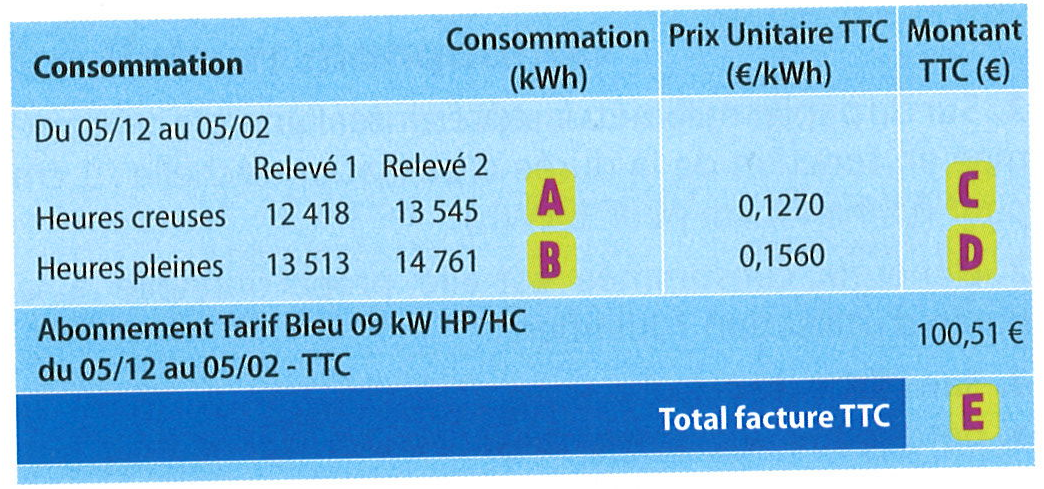
\includegraphics[scale=0.5]{img/facture}
\end{center}

\begin{questions}
	\question Retrouver par le calcul les valeurs manquantes \textbf{A} et \textbf{B}. En déduire les valeurs \textbf{C}, \textbf{D} et \textbf{E}.
	
	\fillwithdottedlines{4cm}
	
	\question Au lieu d'un abonnement <<heures creuses / heures pleines>>, on propose à un client un abonnement de \num{96.50} € avec un prix fixe pour le kWh de \num{0.1449} €. Est-ce plus intéressant ?
	
	\fillwithdottedlines{4cm}
	
	
\end{questions}

\section{Cuisson d'un poulet}

Un four-grill de puissance \num{1500} W permet de cuire un poulet en 1 h 15 min.

\begin{questions}
	\question 	
		\begin{parts}
			\part Rappeler la relation qui permet de calculer l'énergie $E$, consommée par un appareil à partir de sa puissance $P$ et  et sa durée d'utilisation $t$.
			\fillwithdottedlines{1.5cm}
			
			\part Indiquer les unités dans la relation précédente pour que l'énergie soit exprimée en $kWh$.
			\fillwithdottedlines{1.5cm}
		\end{parts}
	
	\question Déterminer l'énergie électrique nécessaire pour la cuisson d'un poulet, en kWh.
	\fillwithdottedlines{3cm}
	
\end{questions}

\section{Consommation de radiateurs}

Une habitation est chauffée par quatre radiateurs électriques portant les indications : 230 V - \num{1.2} kW.

\begin{questions}
	\question Calculer la puissance totale de ces quatre radiateurs en fonctionnement.
	
	\fillwithdottedlines{3cm}
	
	\question Ces radiateurs peuvent-ils être branchés sur une même prise protégée par un disjoncteur de 20 A.
	
	\fillwithdottedlines{3cm}
	
	\question La consommation totale de ces quatre radiateurs est de \num{28.8} kWh. Combien de temps ont-ils fonctionné ?
	\fillwithdottedlines{3cm}
	
	\question Avant d'utiliser les radiateurs, el compteur électrique indique : \num{84237} kWh. Qu'indiquera-t-il 2 mois après si les quatre radiateurs ont fonctionné 8 heures par jour ?
	\fillwithdottedlines{5cm}
	
	\question Sachant que 1 kWh coute environ \num{0.15} € TTC, en déduire le coût d'une telle consommation.
	\fillwithdottedlines{3cm}
\end{questions}








 
%\newpage
%
%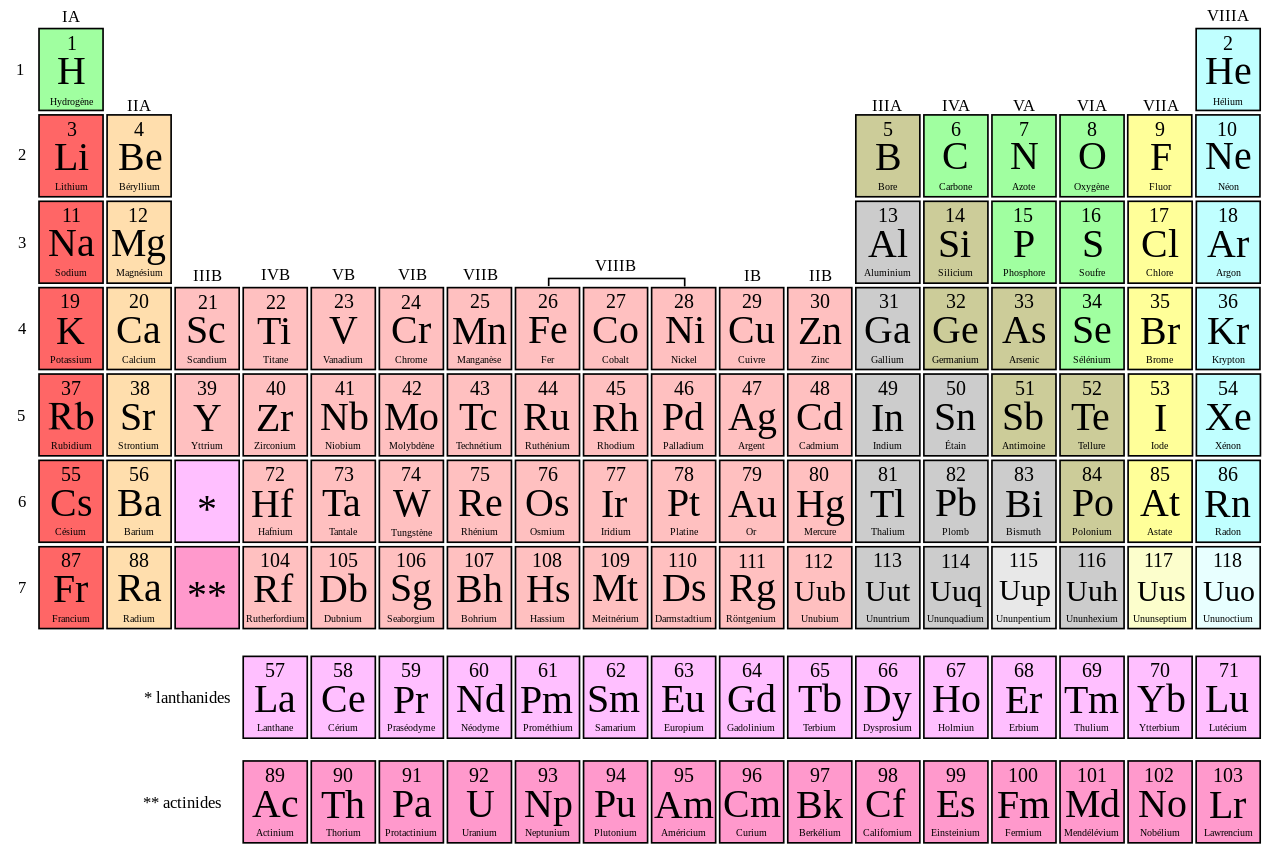
\includegraphics [scale=0.5, angle= 90 ]{img/tableau} 
\ \label{LastPage}

\end{document}